\documentclass[margin 2cm]{report}
\usepackage{indentfirst}
\usepackage{setspace}
\usepackage{graphicx}
\usepackage{float}
\usepackage{url}
\usepackage{subfigure}
\usepackage{geometry}
\geometry{a4paper, scale=0.8}
\setcounter{secnumdepth}{4}
\title{\textbf{Codes and Cryptography Coursework}}
\author{zlqf46, 000785609}
\date{10/1/2021}
\begin{document}
\maketitle
\section[1]{\Large Part one: Compression}
\begin{enumerate}
\normalsize\item[1)]{Number Encoding Int to Byte}
\begin{spacing}{1.5}
\normalsize\indent\setlength{\parindent}{2em}As the LZ series and Huffman are all comming out with the number sequence. And to prevent to write the number to the zip file directly, I Use the function \textbf{int.to\_bytes(number, write\_in\_length, byteorder="big")} to encode the int sequence into the certain bytes length to reduce the length waste, such as encoding the number \textbf{234} into byte b'\verb|\|xea', as the byte width reduce to 1. Which greatly help in compressing number sequence.
\newline Based on the idea behind, the different int number has the different byte length after encoding from int to byte. And the length requirements are as follow:
\newline
\newline
\begin{tabular}{|c|c|c|}
\hline
$255<int<=65535$&$65535<int<=16777215$&$16777215<int$\\
\hline
width 2&width 3&width 4\\
\hline
\end{tabular}
\newline\normalsize\textbf{width 1 if the int smaller than 255}\\
By finding the biggest int number to decide which width is fixed for encoding all int number sequences to reduce the compressing space. Compared to directly encode the number with biggest length (e.g., 4), it can help to make a well organize of the encode byte width to reduce the compressing space.
\end{spacing}

\normalsize\item[2)]{Text file itself to be the search window for LZ-77}
\begin{spacing}{1.5}
\normalsize\indent\setlength{\parindent}{2em}The LZ-77 is a dictionary-based algorithm that encodes long strings (also known as phrases) into short tokens, which replaces phrases in the dictionary with small tokens to achieve the purpose of compression. Which means it compresses data by replacing long strings of repeated occurrences in the data with small symbols. The main idea of LZ-77 is to find repeated characters in the data that has appeared before. In normally, a fixed size search window will be set to reduce the searching time while compressing. But in order to reach the high performance of compressing. There is no limitation of the size of the search window, which means it can search for the repetition through all text file to have a higher performance when compressing the long repeat text than other algorithms.
\end{spacing}

\normalsize\item[3)]{Comparing Compressing}
\begin{spacing}{1.5}
\normalsize\indent\setlength{\parindent}{2em}Different compression algorithms have different compression effects. Thus, I implement 5 algorithms (methods) LZ-77, LZW, Huffman, Hybrid LZW-Huffman and Hybrid LZ77-Huffman. Base on their compression result to choose the final compression method. The advantages of each algorithm are shown below:
\newline\normalsize a) LZ-77:   As the idea \textbf{2)} mentioned, the LZ-77 can have a high performance on compressing the long repeat text file while using other single algorithm.
\newline\normalsize b) Huffman:   Each letter in the text file will be encode into a set of binary arrays and the length of the arrays depends on the frequency (weight) of the  letter in the text file. Each of the binary array was compute from the full binary tree of Huffman tree. Each node corresponds to a letter and the weight of the node is the letter's frequency in the text file. So, this algorithm is different from the others. The Huffman coding is not relying on the order of the letter appear in the text file. Thus, when compressing the small text file or some disorganized text file can have a better performance than others. The code work of the Huffman coding was based on the work from the web \textbf{OmegaXYZ}\footnote[1]{\url{https://www.omegaxyz.com/2018/05/12/huffman_python/}}.
\newline\normalsize c) LZW:   It is called list compression algorithm. In this algorithm, a dictionary of the string will build at first and update the new string with a value to represent, which the value is a number. It is related to the position of the string in the text file and write the number into the compressed file. If the string appears again, it can be replaced by a number (the correspond value in the dictionary) representing it. And the dictionary will not write into the compressed file. In this algorithm, I set up an original dictionary for encoding and decoding (key and value swap position) by using the \textbf{in2byte()} function in \textbf{six} package. This algorithm only needs to write the number into the compressed file and no need to store the dictionary, which can make a high performance (speed and compression rate) in compressing long text file.
\newline Thus, based on the advantages behind (Hybrid LZW-Huffman and LZ77-Huffman algorithms will be mentioned as the idea later). When compressing different kinds of text file, it can first compress by all the algorithms and compare them to choose a shortest one and finished the compression.
\end{spacing}

\normalsize\item[4)]{Hybrid Algorithm}
\begin{spacing}{1.5}
\normalsize\indent\setlength{\parindent}{2em}Base on the ideas \textbf{4) and 5)}, there is no doubt that the LZ series can combine with the Huffman algorithm to make a better performance. That is because the Huffman algorithm is based on the frequency of the character in the text file to encode it (not rely on the order of the text file) and LZ series is focus on the order of the text sequence and the character repetition to compress the text file. Thus, after encoding by the LZ series algorithm, the outcome number sequence may have many repeated number sequences. Then the number sequences can be transfer into the binary string and encode again by Huffman algorithm.
\end{spacing}

\normalsize\item[5)]{Hybrid Algorithm LZW-Huffman}
\begin{spacing}{1.5}
\normalsize\indent\setlength{\parindent}{2em}As I mentioned in section 3). I found a hybrid algorithm called LZW-Huffman which combine the LZW and Huffman together to develop the compression performance. As the LZW encode the text file and save with sequences of number, the number sequence can be replaced by a corresponding character from the dictionary which create by the \textbf{in2byte()} function in \textbf{six} package. Then transfer into a binary string and compressed by Huffman algorithm. But the limitation is the number in the number sequence which encoded by the LZW should be less than 255. So, to solve this problem. Firstly, find out the biggest number in the number sequence, and then compare it with $255$, $255^{2}$, $255^{3}$  and  $255^{4}$. To define whether the number should be separate into the group with one, two, three or more number which smaller than 255. The checklist and corresponding groups are shown below:
\end{spacing}

\begin{figure}[H]
\centering
\label{Fig.sub.1}\includegraphics[height=0.12\textheight,width=0.45\textwidth]{evidence/Hy_example.png}
\caption{the function to dealing the number sequence}
\label{Fig.main}
\end{figure}

\normalsize The \textbf{num} is the biggest number in the number sequence.
\newline
\begin{tabular}{|c||c|c|c|c|}
\hline
Conditions&$0<num<=255$&$255<num<=255^{2}$&$255^{2}<num<=255^{3}$&...\\
\hline
byte width&1&2&3&...\\
\hline
group e.g. number 240&$[240]$&$[240,0]$&$[240,0,0]$&...\\
\hline
group e.g. number 370&None&$[115,1]$&$[115,1,0]$&...\\
\hline
group e.g. number 65770&None&None&$[235,2,1]$&...\\
\hline
\end{tabular}
\newline
\begin{spacing}{1.5}
\newline\normalsize\indent\setlength{\parindent}{2em} After encoding the number sequence with function \textbf{encode\_Hy()} . Because each group of number can have can get a corresponding character from the dictionary, the number can be transformed into a character and combine together as a binary string instead of the number sequence. Then compress by the Huffman algorithm. As I mentioned in the 1st and 2nd idea, the original number sequence from LZW will be encoded with the same byte length depend on the size of the biggest number in the number sequence, which has the same byte width as encoding the number and transfer to corresponding character. But it can be compress again with Huffman algorithm after the transform. Which can help to further compress the text file.
\end{spacing}

\normalsize\item[6)]{Hybrid Algorithm LZ77-Huffman}
\begin{spacing}{1.5}
\normalsize\indent\setlength{\parindent}{2em}Inspired by Hybrid LZW-Huffman algorithm, the compressed LZ-77 can also be compressed by Huffman again using almost the same way as LZW-Huffman in the number transformation. But the little different is LZW comes out with the number sequence and the LZ-77 comes out with the combination of words and two number sequences. Which means I need to add the word together with the two number sequences together to make the binary string for Huffman to compress. Thus, when combining two number sequences, the word use the function \textbf{encode(encoding="ascii")} to encode into the binary string and combine with the encoded binary string transform from the number (as the step in idea \textbf{4)}). Thus, the outcomes of the LZ77 can be compressed again by Huffman algorithm. But different with LZW-Huffman, LZ77-Huffman can make a better compression dealing with the high repeated sequence file. Which means the LZ77-Huffman can have a better performance than LZW-Huffman on files with a high repetition.
\end{spacing}

\end{enumerate}


\newpage
\Large\section[2]{Cryptography}

\begin{enumerate}
\normalsize\item[1)]{Attack Plan}
\begin{spacing}{1.5}
\newline\normalsize\indent\setlength{\parindent}{2em}According to the FAQs\footnote[2]{\url{https://support.what3words.com/en/articles/2212810-what-are-the-shortest-and-longest-words-used}} on the whats3words web page. I found that in English, the shortest words are four letters long and the longest words are 17-18 letters. And when trying the \textbf{encrypt.exe}, I also found that the input length of the Hexadecimal code is the same as the outputs (as shown in the example with "0123456789abcdef"). And the input codes length should be multiple of 8. \newline Mentioned in the coursework requirement, the length of the final outcome of the encryption is 32 bytes. And the key which in the \texbf{encrypt.exe} is the same while encrypting the outcome. \newline Thus, the input length of 3 words location should be 32 bytes after converting to hexadecimal. Each length of the words in the location string should be in range 4 to 18. And the result of the 3 words (in hexadecimal) from \textbf{encrypt.exe} should be the same as using the DES in ECB mode. So, I will try to use the words in the word list to combine a 3 words location (using three 'for' loops) to encrypt it and compare it to the outcome. If it is the same, the location is found. For the coding part, I used the \textbf{multiprocessing.Pool} package. For the first word (in the first 'for' loop), separate the words list in few groups (run it in \textbf{Pool}) to combine with the second word (in the second 'for' loop)  and the third word (in the third 'for' loop). \newline\textbf{Material: 10k words list\footnote[3]{\url{http://www.mit.edu/~ecprice/wordlist.10000}}, 57k words list\footnote[4]{\url{https://raw.githubusercontent.com/dwyl/english-words/master/words_alpha.txt}}}
\end{spacing}

\begin{spacing}{1.5}
\normalsize\item[2)]{Step for Encryption through \textbf{encrypt.exe}}
\newline\normalsize\indent\setlength{\parindent}{2em}a) Encode the three words location (e.g. b'tile.bills.print') from bytes to hexadecimal which achieve the requirement length 32 bytes for \textbf{encrypt.exe}. \newline b) Encrypt the hexadecimal code using \textbf{encrypt.exe} and get the output. \newline c) Compare the output to the outcome from the coursework requirement.
\end{spacing}

\begin{spacing}{1.5}
\normalsize\item[3)]{Additional Finding}
\newline\normalsize\indent\setlength{\parindent}{2em}While encrypting the hexadecimal code. There are two points I found that can help to reduce the words number to reduce the searching time: a) When encoding the 3 words location from byte (e.g. b'tile.bills.print') to hexadecimal, the length of the hexadecimal code is twice the 3 words location. b) While encrypting through the \textbf{encrypt.exe}, the first 16 bytes of the outcome are the same if the first 8 letters (including the '.') are the same in the 3 words location. \newline\normalsize\indent\setlength{\parindent}{2em}According to the findings above and previous in Attack Plan. Firstly, the length condition for word chosen in 3 words location change to range 4 to 6. As the minimum word's length is 4 and the  of the location should be exactly 16 (to require the 32 bytes length for hexadecimal and outcome), the longest word should no more than $16-2-4-4=6$\footnote[5]{which 2 for two '.', and 4 for the minimum length of the other two words}. Secondly, the searching area can be reduced by finding the first two words (reduce to two 'for' loops, randomly chose the third words) to compare the first 16 bytes of the encryption first. Then find out the first two words and use them to combine each word in words list (one 'for' loop) to find out the final word.
\end{spacing}

\begin{spacing}{1.5}
\normalsize\item[4)]{Attack}
\newline\normalsize\indent\setlength{\parindent}{2em}I first try with the 10k words list because it is the shortest one can finished earlier. By limited the 10k words list with the conditions behind, the number of the words can be reduced to 4k+8 words. So, I separate it into 5 groups for the first loop (5 groups run in parallel using Core i7-9700K 8-core CPU with 16GB RAM on my Windows Laptop). After 280479s (around three days), the output of the first step are three combinations of the location, they are  \textbf{"tile.bill.crimes", "tile.bills.catch","tile.billy.spies"}. \newline Then in the second step, use the word "tile" as the first word. Combine the word "bill" with 1504 words (length 6), "bills" with 1379 words (length 5), "billy" with 1379 words (length 5) which totally $1504+2\times1379=4262$ searches to encrypted by \textbf{encrypt.exe} and compare the outcome string. Fortunately, the 10k words list contain the third word "print" and the final answer for the 3 words is \textbf{"tile.bills.print"}.
\newline\textbf{The total running time is around 280479s+298s=281320s (78 hours). The total searches for the word are $4008^2+4262=16076088$. And the exactly location shows on Google Maps is: 7346 Melrose St, Philadelphia, PA 19136 US}
\end{spacing}

\begin{figure}[H]
\centering
\subfigure[first step time taken]{\label{Fig.sub.1}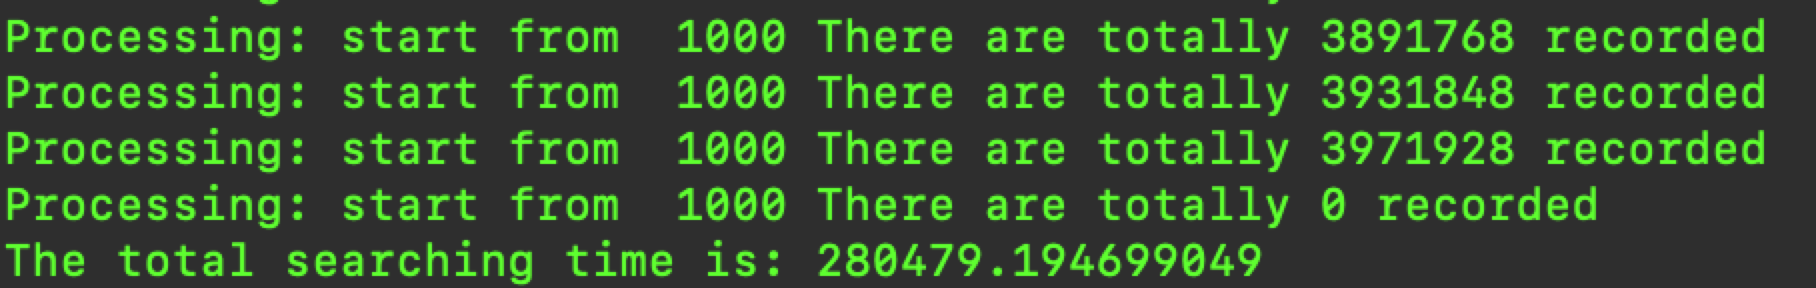
\includegraphics[width=0.5\textwidth]{evidence/time_taken_first_step.png}}
\subfigure[first step result]{\label{Fig.sub.2}\includegraphics[width=0.5\textwidth]{evidence/final_words.png}}
\subfigure[final result]{\label{Fig.sub.3}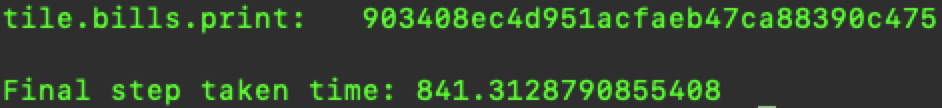
\includegraphics[width=0.5\textwidth]{evidence/final_location.png}}
\caption{Evidence}
\label{Fig.main}
\end{figure}

\normalsize\item[5)]{Evaluation and Fun Facts}
\newline\normalsize\indent\setlength{\parindent}{2em}As I found for reducing the words by the length limitation. There still have some improve in the first step like combining the words in a certain groups with certain length which can meet the length requirement of the 3 words location. And after finding out the 3 words location. I found that the \textbf{encrypt.exe} can be unpacked and find the key inside the \textbf{encrypt} file. Which is \texbf{'98a1bef23455dc03'}. And it works for encrypting the 3 words location with using the Des package in python.
\end{enumerate}


\end{document}